\documentclass[12pt]{report}

%%%%%%%%%%%%%%%%%%%%%%%%%%
%%%%%% UNIT PREAMBLE %%%%% 
%%%%%%%%%%%%%%%%%%%%%%%%%%

% Basics 
\usepackage[utf8]{inputenc}
\usepackage[T1]{fontenc}
\usepackage{textcomp}
\usepackage[a4paper, left=1in, right=1in, top=1in, bottom=1in]{geometry}
\renewcommand\familydefault{\sfdefault}

\usepackage[Sonny]{fncychap}

\usepackage{amsmath,amsfonts,amsthm,amssymb,mathtools}
\usepackage[varbb]{newpxmath}
\usepackage{xfrac}
\usepackage[usenames,dvipsnames]{xcolor} % usenames, dvipsnames adds more colours
\usepackage{hhline}
\usepackage{comment}
\usepackage{tasks}
\usepackage{enumerate} 
\usepackage{enumitem} 
\usepackage{titlesec}
\usepackage[most]{tcolorbox}
\usepackage{lipsum}
\usepackage{tabularx}
\usepackage[labelfont=bf]{caption}
\usepackage{subfig}
\usepackage{pgfplots}
\usepackage{cancel} 
\usepackage{physics} 
\usepackage[bookmarks]{hyperref}
\usepackage{array}
\usepackage{float}
\usepackage{standalone}
\usepackage{graphicx}
\usepackage{forest}

% Tables 
\numberwithin{table}{section}

% Inkscape Figures
\usepackage{import}
\usepackage{xifthen}
\usepackage{pdfpages}
\usepackage{transparent}
\newcommand{\incfig}[2][1]{
    \def\svgwidth{#1\columnwidth}
    \import{../figures/}{#2.pdf_tex}
}

\pdfsuppresswarningpagegroup=1

% Chemistry
\usepackage{lewis} 
\usepackage{bohr}
\usepackage[version=4]{mhchem}

% Page setup
\hypersetup{hidelinks}
\pagenumbering{arabic}
\pagestyle{plain}
\setlength{\parindent}{0pt}

% Show subsubsections
\setcounter{tocdepth}{3}
\setcounter{secnumdepth}{3}

% Required for the Grid
\usetikzlibrary{calc}

% Section Font-Size
\titleformat{\subsubsection}
  {\normalfont\fontsize{12}{12}\bfseries}{\thesubsubsection}{1em}{}

\titleformat{\subsection}
  {\normalfont\fontsize{14}{14}\bfseries}{\thesubsection}{1em}{}

\titleformat{\section}
  {\normalfont\fontsize{16}{16}\bfseries}{\thesection}{1em}{}

% New page for each section 
\newcommand{\sectionbreak}{\clearpage}

% Section Spacing
\titlespacing{\section}{0em}{2.5em}{1em}
\titlespacing{\subsection}{0em}{2.5em}{1em}
\titlespacing{\subsubsection}{0em}{2.5em}{1em}

% TABLE COLUMN SEPARATION (USES ARRAY PACKAGE)
% \renewcommand{\arraystretch}{1.8} % changes vertical space for each cell 
% \setlength{\tabcolsep}{18pt} % changes horizontal space for each cell
% \setlength{\arrayrulewidth}{0.25mm}

% TCOLORBOX 
% \newtcolorbox[auto counter, number within=section]{definition}{colback=white,title=Example~\thetcbcounter,breakable,colframe=white,boxrule=0pt, enhanced, title style={left color=gray!60,right color=white,middle color=white},arc=0mm, titlerule=0pt, fonttitle=\bfseries\sffamily}

% Theorems 
\usepackage{thmtools}
\usepackage[framemethod=TikZ]{mdframed}

\declaretheoremstyle[
    headfont=\bfseries\sffamily\color{ProcessBlue!70!black}, bodyfont=\normalfont,
    headpunct= :,
    mdframed={
        linewidth=2pt,
        rightline=false, topline=false, bottomline=false,
        linecolor=ProcessBlue, backgroundcolor=ProcessBlue!5,
        innerbottommargin=10pt
    } ]{note}

\declaretheoremstyle[
    headfont=\bfseries\sffamily\color{NavyBlue!70!black}, 
    bodyfont=\normalfont,
    % headpunct=,
    mdframed={
        linewidth=2pt,
        rightline=false, topline=false, bottomline=false, linecolor=NavyBlue, innerbottommargin=10pt
    }
]{solution}

\declaretheoremstyle[
    headfont=\bfseries\sffamily\color{Gray!70!black}, bodyfont=\normalfont,
    % headpunct= ,
    postheadspace=\newline,
    mdframed={
        linewidth=2pt,
        rightline=false, topline=false, bottomline=false,
        linecolor=Gray, backgroundcolor=Gray!5,
        innerbottommargin=10pt
    } ]{remark}

\declaretheoremstyle[
    headfont=\bfseries\sffamily\color{Fuchsia!70!black}, bodyfont=\normalfont,
    % headpunct= ,
    mdframed={
        linewidth=2pt,
        rightline=false, topline=false, bottomline=false,
        linecolor=Fuchsia, backgroundcolor=Fuchsia!5,
        innerbottommargin=10pt
    }
]{example}

\declaretheoremstyle[
    headfont=\bfseries\sffamily\color{Fuchsia!70!black}, 
    bodyfont=\normalfont,
    % headpunct= ,
    mdframed={
        linewidth=2pt,
        rightline=false, topline=false, bottomline=false,
        linecolor=Fuchsia,
    }
]{examplesolution}

\declaretheoremstyle[
    headfont=\bfseries\sffamily\color{black!70!black}, 
    bodyfont=\normalfont,
    mdframed={
        linewidth=1pt,
        rightline=false, topline=false, bottomline=false,
        linecolor=black,
    }
]{definition}

\declaretheorem[style=solution, name=Solution, numbered=no]{solution}

\declaretheorem[style=solution, name=Derivation, numbered=no]{derivation}

\declaretheorem[style=definition, name=Definition, numberwithin=chapter]{definition}

\declaretheorem[style=note, name=Note, numbered=no]{noteswap}
\newenvironment{note}[1]{\vspace{0.5em}\begin{noteswap}[#1]}{\end{noteswap}\vspace{0.5em}}

\declaretheorem[style=remark, name=Remark, numbered=no]{remarkswap}
\newenvironment{remark}{\vspace{0.5em}\begin{remarkswap}}{\end{remarkswap}\vspace{0.5em}}

\declaretheorem[style=example, name=Example, numbered=no]{exampleswap}
% \newenvironment{example}{\vspace{0.5em}\begin{exampleswap}}{\end{exampleswap}}

\declaretheorem[style=examplesolution, name=Solution, numbered=no]{examplesolutionswap}
\newenvironment{examplesolution}{\vspace{-2em}\begin{examplesolutionswap}}{\end{examplesolutionswap}}

% Enumerate environments 
\newenvironment{2qu}
{
\begin{enumerate}[label=(\alph*)]
}
{\end{enumerate}}

\newenvironment{3qu}
{
\begin{enumerate}[label=(\roman*)]
}
{\end{enumerate}}

% Normal Environments 
\newenvironment{list0.5}
{
\begin{enumerate}
\setlength\itemsep{0.5em}
}
{\end{enumerate}}

% \titleformat{\section}{\vbox{\rule{\linewidth}{0.8pt}}\bigskip\LARGE\bfseries}{\thesection}{1em}{}

\titleformat{\section}
  {\normalfont\Large\bfseries}{\thesection}{1em}{}[{\titlerule[0.8pt]}] % horizontal line below

% thmtools Environments
\newenvironment{problems}
{
    \subsection{Problems}
    \begin{enumerate}
    \setlength\itemsep{1em}
}
{\end{enumerate}}

\newenvironment{+problems}
{
    \subsubsection{Problems}
    \begin{enumerate}
    \setlength\itemsep{1em}
}
{\end{enumerate}}

\newenvironment{example}[1]
{
    \begin{exampleswap}
        #1
    \end{exampleswap}
    \begin{examplesolution}
}
{
\end{examplesolution}}

\newenvironment{2example}[1]
{
    \begin{exampleswap}[#1]
}
{
\end{exampleswap}}

% Managing Figures
\captionsetup{width=0.8\textwidth}
\renewcommand{\thefigure}{\arabic{chapter}.\arabic{figure}}

% TABLE
% \begin{table}[h!] % delete [h!] if there are bugs

%     %%% TABLE CONFIG %%% 
%     \renewcommand{\arraystretch}{1.5} % changes vertical space for each cell 
%     \setlength{\tabcolsep}{10pt} % changes horizontal space for each cell
%     \setlength{\arrayrulewidth}{0.25mm}

%     \begin{center}
%          title of the table \
%         \vspace{0.5em}
%         \begin{tabular}{|c|c|} % use r, l, c for right, left, center. use m{3cm} for middle width of 3cm, use  b{3cm} for bottom width of 3cm, and use p{3cm} for a top width of 3cm.  
%         \hline
%          &  \ % two columns corresponding to two c's
%         \hline
%          &  \ % second row
%         \hline
%         \end{tabular}
%     \end{center}
%     \caption{}
% \end{table}

% Symbols 
\newcommand{\z}{\mathbb{Z}}

\renewcommand{\l}{\ell}

% Formatting 
\newcommand{\invis}{\vphantom{Invisible Text}}
\newcommand{\divider}{\par\noindent\rule{\textwidth}{0.5pt}\vspace{0.4em}}

% Chemistry
% \newcommand{\2ch}[2]{\ce{#1}_{(#2)}}
% \newcommand{\io}[2]{\text{#1}^{#2}} 
% \newcommand{\2io}[3]{\text{#1}^{#2}_{#3}}


\begin{document}

\section{Page 25 (Organelles)}
\begin{enumerate}
\setlength\itemsep{1em}
    \item{What five life processes do cells perform?}
        \begin{solution}
            The five life processes are: 
            \begin{list0.5}
                \item{Metabolism}
                \item{Growth}
                \item{Reproduction}
                \item{Response to stimuli}
                \item{Homeostasis}
            \end{list0.5}
        \end{solution}

    \item{List the five organelles that are common to plant and animal cells. What are their functions?}
        \begin{solution}
            The five common organelles are: 
            \begin{itemize}
                \item{\textbf{Nucleus}: the control center of the brain. Contains the genetic material in the form of DNA to the cell.}
                \item{\textbf{Cell membrane}: a semi-permeable membrane that protects the inner contents of the cell from the outer world.}
                \item{ \textbf{Cytoplasm}: a gel-like substance that suspends the remaining organelles. Provides water and nutrients.}
                \item{ \textbf{Mitochondria}: the powerhouse of the cell. Converts stored energy into usuable energy through cellular respiration (more folds means more energy).}
                \item{ \textbf{Golgi apparatus/body}: acts as a post-office in the cell. Collects materials from the ER and processes them for removal from the cell.}
            \end{itemize}
        \end{solution}

    \item{What are three differences between plant and animal cells?}
        \begin{solution}
            The plant cell contains (whereas the animal cell doesn't): 
            \begin{itemize}
                \item{Chloroplast}
                \item{Cell wall}
                \item{Large central vacuole}
            \end{itemize}
        \end{solution}

    \item{Why can the granum and thylakoid structures be described as ``solar collectors''?}
        \begin{solution}
            A stack of thylakoids is known as a granum. Each thylakoid uses energy from the sun to photosynthesize it into energy, hence the nickname ``solar collectors''.\\ 

        Specifically, they are responsible for capturing energy and converting light energy from the sun into chemical energy in the form of ATP, which is used in photosynthesis.\\ 

        The thylakoid membranes contain pigments, including chlorophyll, that are able to absorb light energy from the sun. This energy is then used to power the process of photosynthesis, which involves the conversion of carbon dioxide and water into glucose and oxygen.
        \end{solution}

    \item{Prepare a table that summarizes the organelles and structures found in plant and animal cells.}

    \item{Explain how fluorence microscopy works.}

    \item{Name two types of electron microscopes that are used by cell biologists.}

    \item{What is the name of the image created by an electron microscope?}

    \item{Explain the importance of contrast in microscopy.}

    \item{What two things can you do to create contrast when you use a compound light microscope to study a specimen?}

    \item{Think about the function of the mitochondria. You have been asked to view cells taken from the leg muscle of an athlete and cells taken from the skin of an elderly individual. What differences in the number of mitochondria would you see in the two samples? Explain your thinking.}
        \begin{solution}
            Obviously there would be more mitochondria in the leg muscle of an athlete as opposed to that of an elderly individual. The elderly individual just has dead cells and hence dead mitochondria.
        \end{solution}

    \item{Explain how a microscope may be used to assess human health.}

    \item{Write a short paragraph that compares and contrasts plant and animal cells by considering structures, presence of specialized compounds, and forms of energy storage.}
\end{enumerate}

\section{Page 37 (Cell Cycle)}
\begin{enumerate}
\setlength\itemsep{1em}
    \item{Describe the events in the cell cycle.}
        \begin{solution}
            The stages are listed below along with their phases 
            \begin{itemize}
                \item{ \textbf{Interphase}}
                    \begin{itemize}
                        \item{G1 phase: regular cell functions.}
                        \item{S phase: DNA is replicated.}
                        \item{G2 phase: organelles are duplicated; prepartion for mitosis.}
                    \end{itemize}
                \item{ \textbf{Mitosis}}
                    \begin{itemize}
                        \item{Prophase: chromosomes condense. They shorten and thicken.}
                        \item{Metaphase: the chromosomes line up in the middle of the nucleus. The two sister chromatids are linked together by centromere.}
                        \item{Anaphase: the centromere breaks and the sister chromatids split apart.}
                        \item{Telophase: two nuclei formed after nuclear envelopes reform around each group of chromosomes.}
                    \end{itemize}
                \item{\textbf{Cytokinesis}: the cytoplasm is split and two daughter cells are born. In an animal cell, this is done through the pinching of the membrane (cleavage furrow) and in a plant cell, this is done through the formation of the cell plate.}
            \end{itemize}
        \end{solution}

        \item{Describe the meaning of the term ``apoptosis'' and state its importance.}
            \begin{solution}
                Apoptosis is used to describe a cell that is ``self-destructing''. 
            \end{solution}

        \item{State one similarity and one difference between plant and animal mitosis.}

        \item{What is a cancer cell?}
            \begin{solution}
                A cancer cell is a cell that grows and divides uncontrollably. This leads to visible tumors around the body. Cancer cell are formed by genetic mutations amongst normal cells.  
            \end{solution}

        \item{Ensure how mitosis ensures genetic continuity.}
            \begin{solution}
                During mitosis, the chromosomes are duplicated into sister chromatids, and hence the genetic information is preserved.
            \end{solution}

        \item{How does mitosis make the growth and repair of cells possible in an organism?}
            \begin{solution}
                The telophase phase of mitosis is when the cytoplasm is split in half and two daughter cells are formed. This ensures that cells are reborn and the more cells, the greater the surface area to volume ratio, and hence the greater the growth.
            \end{solution}

        \item{Why would you expect cells to spend the greatest percentage of their cycle in interphase?}
        \begin{solution}
            During interphase, the cell spends most of its cell functions, including growth, metabolis, and DNA replication for cell division. In other words, interphase is the period in which the cell grows, which obviously takes time.
        \end{solution}

        \item{What happens to the chromosomes as a cell prepares to divide?}
            \begin{solution}
                The chromosomes condenses and eventually forms daughter chromatids which is then split into their individual cell nuclei when the cytoplasm splits.
            \end{solution}

        \item{How is a cancer cell different from a normal cell? Give three differences.}
            \begin{solution}
                Three differences are listed below: 
                \begin{itemize}
                    \item{Cancer cells do not stop reproducing.}
                    \item{May move to another location of the body.}
                    \item{Does not stick to other cells. Behaves independently.}
                \end{itemize}
            \end{solution}

        \item{Describe the differences between mitosis in an animal cell and a plant cell.}
            \begin{solution}
                In an animal cell, the cytoplasm splits through cleavage furrow whereas the plant cell splits by forming a cell plate.
            \end{solution}

        \item{Why must cell division be controlled or regulated for cells to remain healthy? Explain your answer.}
            \begin{solution}
                If cell division is not properly controlled, cells can become damaged or mutated, leading to the formation of cancer and other diseases.
            \end{solution}

        \item{A certain antibiotic affects cells by preventing the formation of spindle fibres. Explain how this drug would affect mitosis in cells.}

        \item{A drug used in chemotherapy causes chromosomes to move incorrectly during mitosis. As a result, the daughter cells that are produced have either too much or too little genetic information. Predict why this treatment causes the cancer cells to die.}

        \item{15. Identify the stage of mitosis shown in the photo below. Explain your thinking.}
            \begin{solution}
                This is the anaphase stage of mitosis, when the centromeres break off andthe sister chromatids are pulled back.
            \end{solution}

            \begin{figure}[H]
            \centering
                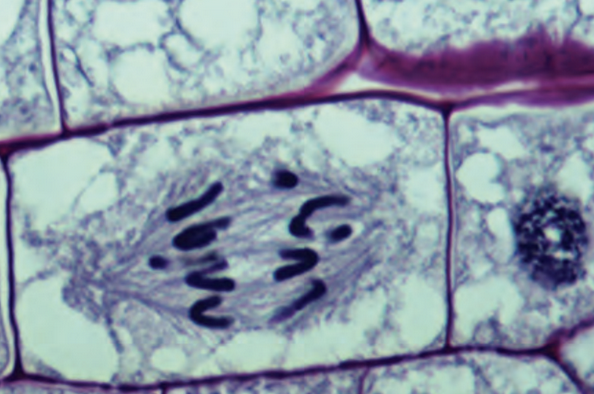
\includegraphics[width=0.5 \textwidth ]{../figures/mitosis problem.png}
                \label{fig:}
            \end{figure}

        \item{The nerve cells in our bodies rarely undergo mitosis. Use this information to explain why complete recovery from injuries to our nervous system may not occur.}
            \begin{solution}
                If nerve cells in our bodies rarely undergo mitosis, then the nerve cells cannot be reproduced. Hence, once nerve cells die, they are gone forever.
            \end{solution}

        \item{Sunscreens protect your skin by blocking types of ultraviolet radiation. Explain why the Canadian Cancer Society advises Canadians to apply sunscreen.}
            \begin{solution}
                Reduces risk of genetic mutations within cells and hence lower chance of cancer.
            \end{solution}

        \item{Suggest reasons why cancer researchers may be interested in using their learning about the processes of cell division to develop new forms of cancer prevention and treatment.}
            \begin{solution}
                They can perhaps limit the ways that the cancer cells divide. 
            \end{solution}

        \item{Three samples of cells from three different patients were unlabelled. One sample was from an 85-year-old man, one was from a 5-year-old boy, and one was from a person with skin cancer. How could you determine to which patient they belonged?}
            \begin{solution}
                The one with the least cells is the old person, the one with the second least cells is the 5-year-old boy, and the one with the most is from the person with skin cancer.
            \end{solution}
\end{enumerate}

\end{document}
